\documentclass[12pt, notitlepage, final]{article}

\newcommand{\name}{Vince Coghlan}

%\usepackage[dvips]{graphics,color}
\usepackage{amsfonts}
\usepackage{amssymb}
\usepackage{amsmath}
\usepackage{latexsym}
\usepackage{enumerate}
\usepackage{amsthm}
\usepackage{nccmath}
\usepackage{setspace}
\usepackage[pdftex]{graphicx}
\usepackage{epstopdf}
\usepackage[siunitx]{circuitikz}
\usepackage{tikz}
\usepackage{float}
\usepackage{cancel}
\usepackage{setspace}
\usepackage{overpic}
\usepackage{mathtools}
\usepackage{listings}
\usepackage{color}
\usepackage{qtree}
%\usepackage{gensymb}

\usetikzlibrary{calc}
\usetikzlibrary{matrix}
\usetikzlibrary{positioning}

\numberwithin{equation}{section}
\DeclareRobustCommand{\beginProtected}[1]{\begin{#1}}
\DeclareRobustCommand{\endProtected}[1]{\end{#1}}
\newcommand{\dbr}[1]{d_{\mbox{#1BR}}}
\newtheorem{lemma}{Lemma}
\newtheorem*{corollary}{Corollary}
\newtheorem{theorem}{Theorem}
\newtheorem{proposition}{Proposition}
\theoremstyle{definition}
\newtheorem{define}{Definition}
\newcommand{\column}[2]{
\left( \begin{array}{ccc}
#1 \\
#2
\end{array} \right)}

\newdimen\digitwidth
\settowidth\digitwidth{0}
\def~{\hspace{\digitwidth}}

\setlength{\parskip}{1pc}
\setlength{\parindent}{0pt}
\setlength{\topmargin}{-3pc}
\setlength{\textheight}{9.0in}
\setlength{\oddsidemargin}{0pc}
\setlength{\evensidemargin}{0pc}
\setlength{\textwidth}{6.5in}
\newcommand{\answer}[1]{\newpage\noindent\framebox{\vbox{{\bf ECEN 5018 Spring 2014} 
\hfill {\bf \name} \vspace{-1cm}
\begin{center}{Midterm}\end{center} } }\bigskip }

\DeclareMathOperator*{\argmin}{arg\,min}

%absolute value code
\DeclarePairedDelimiter\abs{\lvert}{\rvert}%
\DeclarePairedDelimiter\norm{\lVert}{\rVert}
\makeatletter
\let\oldabs\abs
\def\abs{\@ifstar{\oldabs}{\oldabs*}}
%
\let\oldnorm\norm
\def\norm{\@ifstar{\oldnorm}{\oldnorm*}}
\makeatother

\def\dbar{{\mathchar'26\mkern-12mu d}}
\def \Frac{\displaystyle\frac}
\def \Sum{\displaystyle\sum}
\def \Int{\displaystyle\int}
\def \Prod{\displaystyle\prod}
%\def \P[x]{\Frac{\partial}{\partial x}}
%\def \D[x]{\Frac{d}{dx}}
\newcommand{\PD}[2]{\frac{\partial#1}{\partial#2}}
\newcommand{\PF}[1]{\frac{\partial}{\partial#1}}
\newcommand{\DD}[2]{\frac{d#1}{d#2}}
\newcommand{\DF}[1]{\frac{d}{d#1}}
\newcommand{\fix}[2]{\left(#1\right)_#2}
\newcommand{\ket}[1]{|#1\rangle}
\newcommand{\bra}[1]{\langle#1|}
\newcommand{\braket}[2]{\langle #1 | #2 \rangle}
\newcommand{\bopk}[3]{\langle #1 | #2 | #3 \rangle}
\newcommand{\Choose}[2]{\displaystyle {#1 \choose #2}}
\newcommand{\proj}[1]{\ket{#1}\bra{#1}}
\def\del{\vec{\nabla}}
\newcommand{\avg}[1]{\langle#1\rangle}
\newcommand{\piecewise}[4]{\left\{\beginProtected{array}{rl}#1&:#2\\#3&:#4\endProtected{array}\right.}
\newcommand{\systeme}[2]{\left\{\beginProtected{array}{rl}#1\\#2\endProtected{array}\right.}
\def \KE{K\!E}
\def\Godel{G$\ddot{\mbox{o}}$del}

%\onehalfspacing

\begin{document}

\answer{}

\textbf{1)} One role for learning algorithms in distributed control is to guide the decisions of players in real time.
However, in many settings players may not have the ability to select any particular action in their action set at any
given time.  For example consider the problem of multi-vehicle motion control where an agent's action set represents
discrete spatial locations.  Here, mobility limitations restrict the ability to traverse from one location to another
in a given time period.

To formalize this notion of constrained action sets, consider the following process: Let $a(t-1)$ be the joint action
at time $t-1$.  With constrained action sets, the set of actions available to player $i$ at time $t$ is a function of
his action at time $t-1$ and will be denoted as $C_i(a_i(t-1)) \subseteq \mathcal{A}_i$.  For example, consider the
following two player identical interest game with payoffs
\begin{center}
\begin{tabular}{r |c|c|c|}
  \multicolumn{1}{r}{}
  & \multicolumn{1}{c}{$b_1$}
  & \multicolumn{1}{c}{$b_2$}
  & \multicolumn{1}{c}{$b_3$}\\
  \cline{2-4}
  $a_1$ & 0,0 & 0,0 & 9,9\\
  \cline{2-4}
  $a_2$ & 10,10 & -10,-10 & -10,-10\\
  \cline{2-4}
\end{tabular}
\end{center}
and constrained action sets that satisfy
\[
  C_1(a_1)=\{a_1,a_2\}, C_1(a_2)=\{a_1,a_2\}
\]
\[
  C_2(b_1)=\{b_1,b_2\}, C_2(b_2)=\{b_1,b_2,b_3\}, C_2(b_3)=\{b_2,b_3\}
\]
Standard log-linear learning assumes an agent can access any action at each iteration, i.e., $C_i(a_i)=\mathcal{A}_i$
for all actions $a_i \in \mathcal{A}_i$.  The goal of this problem is to understand how mobility limitations impact
the resulting behavior associated with log-linear learning.  Here, we now consider two variations of log-linear learning
which can accommodate constrained action sets.

\begin{itemize}
  \item{\textbf{Variation \#1:} At each time $t$, the updating player $i$ plays a stragey $p_i(t)\in\Delta(\mathcal{A}_i)$ where}
  \[
  p_i^{a_i}(t)=\left\{ \begin{array}{l r} \frac{e^{\frac{1}{\tau} U_i(a_i,a_{-i}(t-1))}}{\sum_{\tilde{a}_i\in C_i(a_i)}e^{\frac{1}{\tau} U_i(\tilde{a}_i,a_{-i}(t-1))}} & \text{for any action $a_i\in C_i(a_i(t-1))$} \\ 0 & \text{for any action $a_i \notin C_i(a_i(t-1))$} \end{array} \right.
  \]
\item{\textbf{Variation \#2:} At each time $t$, the updating player $i$ selects one trial action $\tilde{a}_i$ (uniformly) from
  his constrained action set $C_i(a_i(t-1)) \subset \mathcal{A}_i$.  Player $i$ plays a strategy $p_i(t) \in \Delta(A_i)$ where}
  \[
  p_i^{a_i}(t)=\left\{ \begin{array}{l r} \frac{e^{\frac{1}{\tau} U_i(a_i,a_{-i}(t-1))}}{\sum_{\bar{a}_i\in\{a_i(t-1),\tilde{a}_i\}}e^{\frac{1}{\tau} U_i(\bar{a}_i,a_{-i}(t-1))}} & \text{for any action $a_i\in \{a_i(t-1),\tilde{a}_i\}$} \\ 0 & \text{for any action $a_i \notin \{a_i(t-1),\tilde{a}_i\}$} \end{array} \right.
  \]
\end{itemize}

\begin{enumerate}
  \item{Characterize the behavior of log-linear learning with Variation \#1 as $\tau\rightarrow 0^+$ for the
    above example.}\\
  In this strategy, each player picks based on each action that they can take at that time.  It should be noted
  that for player 1, this will always act like the normal log-linear learning.  For player 2, however, this can change.
  As $\tau \rightarrow 0$ the equilibria chosen depends on the initial position, since once you end up somewhere,
  you stay there.  For example, these two plots were made when $\tau$ was relatively high ($\tau=5$):
  \begin{figure}[H]
  \begin{center}
  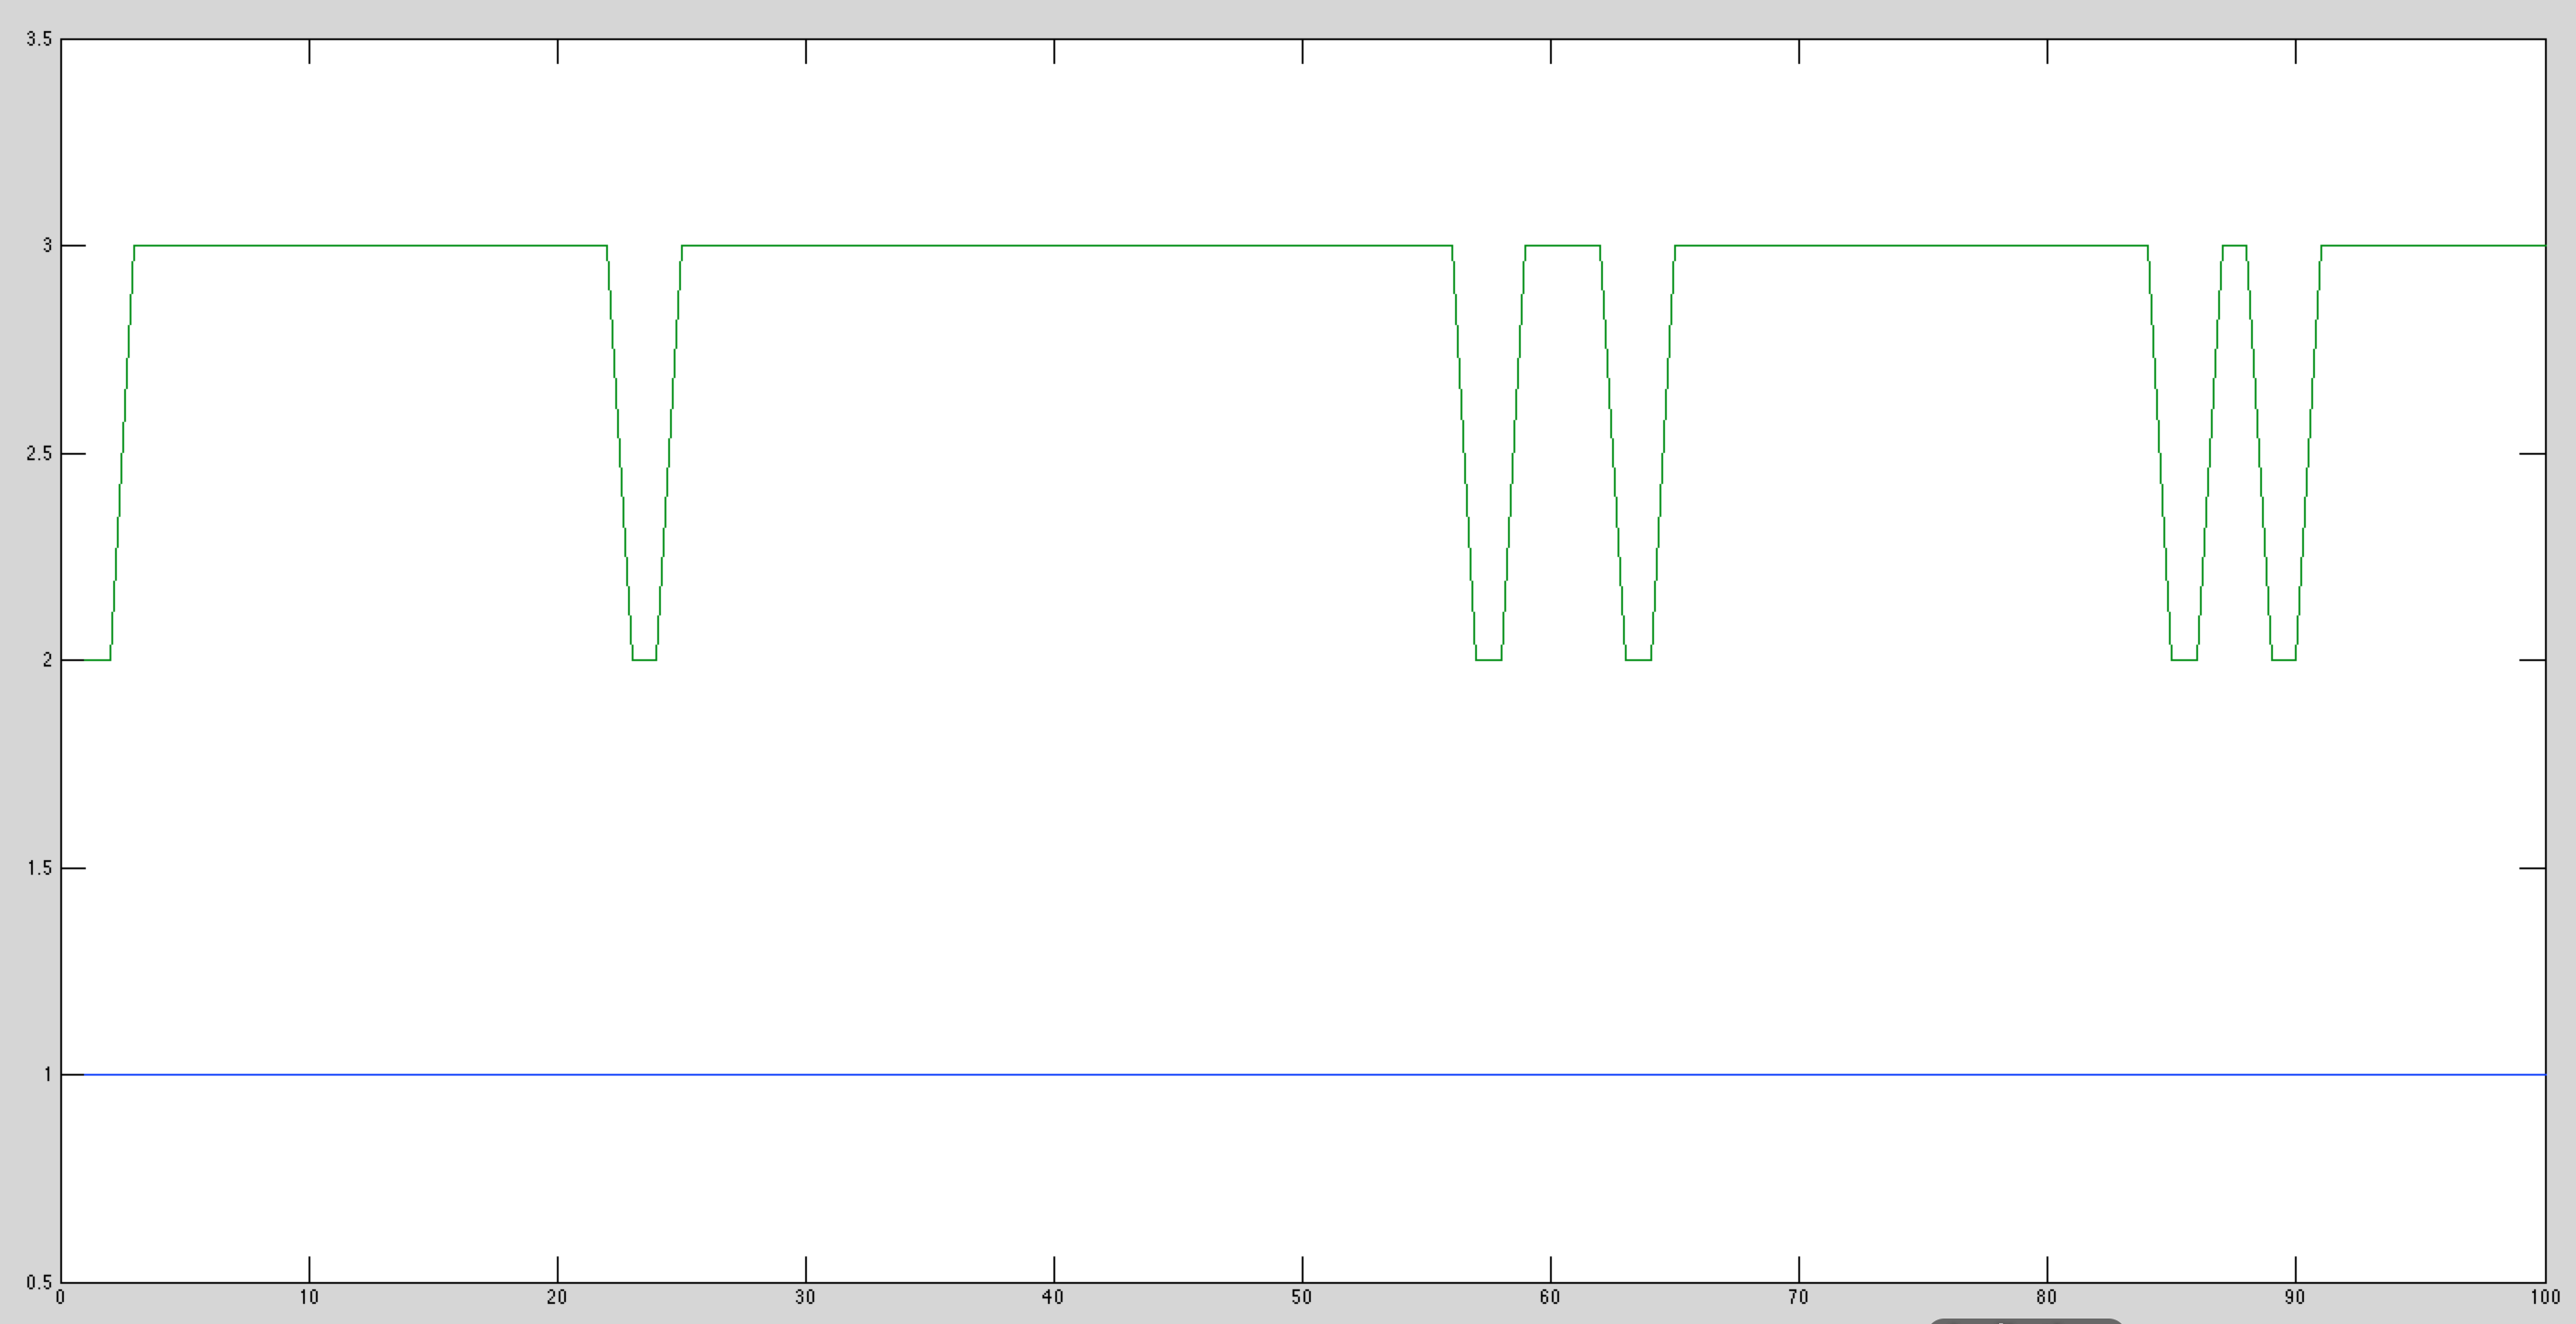
\includegraphics[width=14cm]{f1}
  \end{center}
  \end{figure}
  \begin{figure}[H]
  \begin{center}
  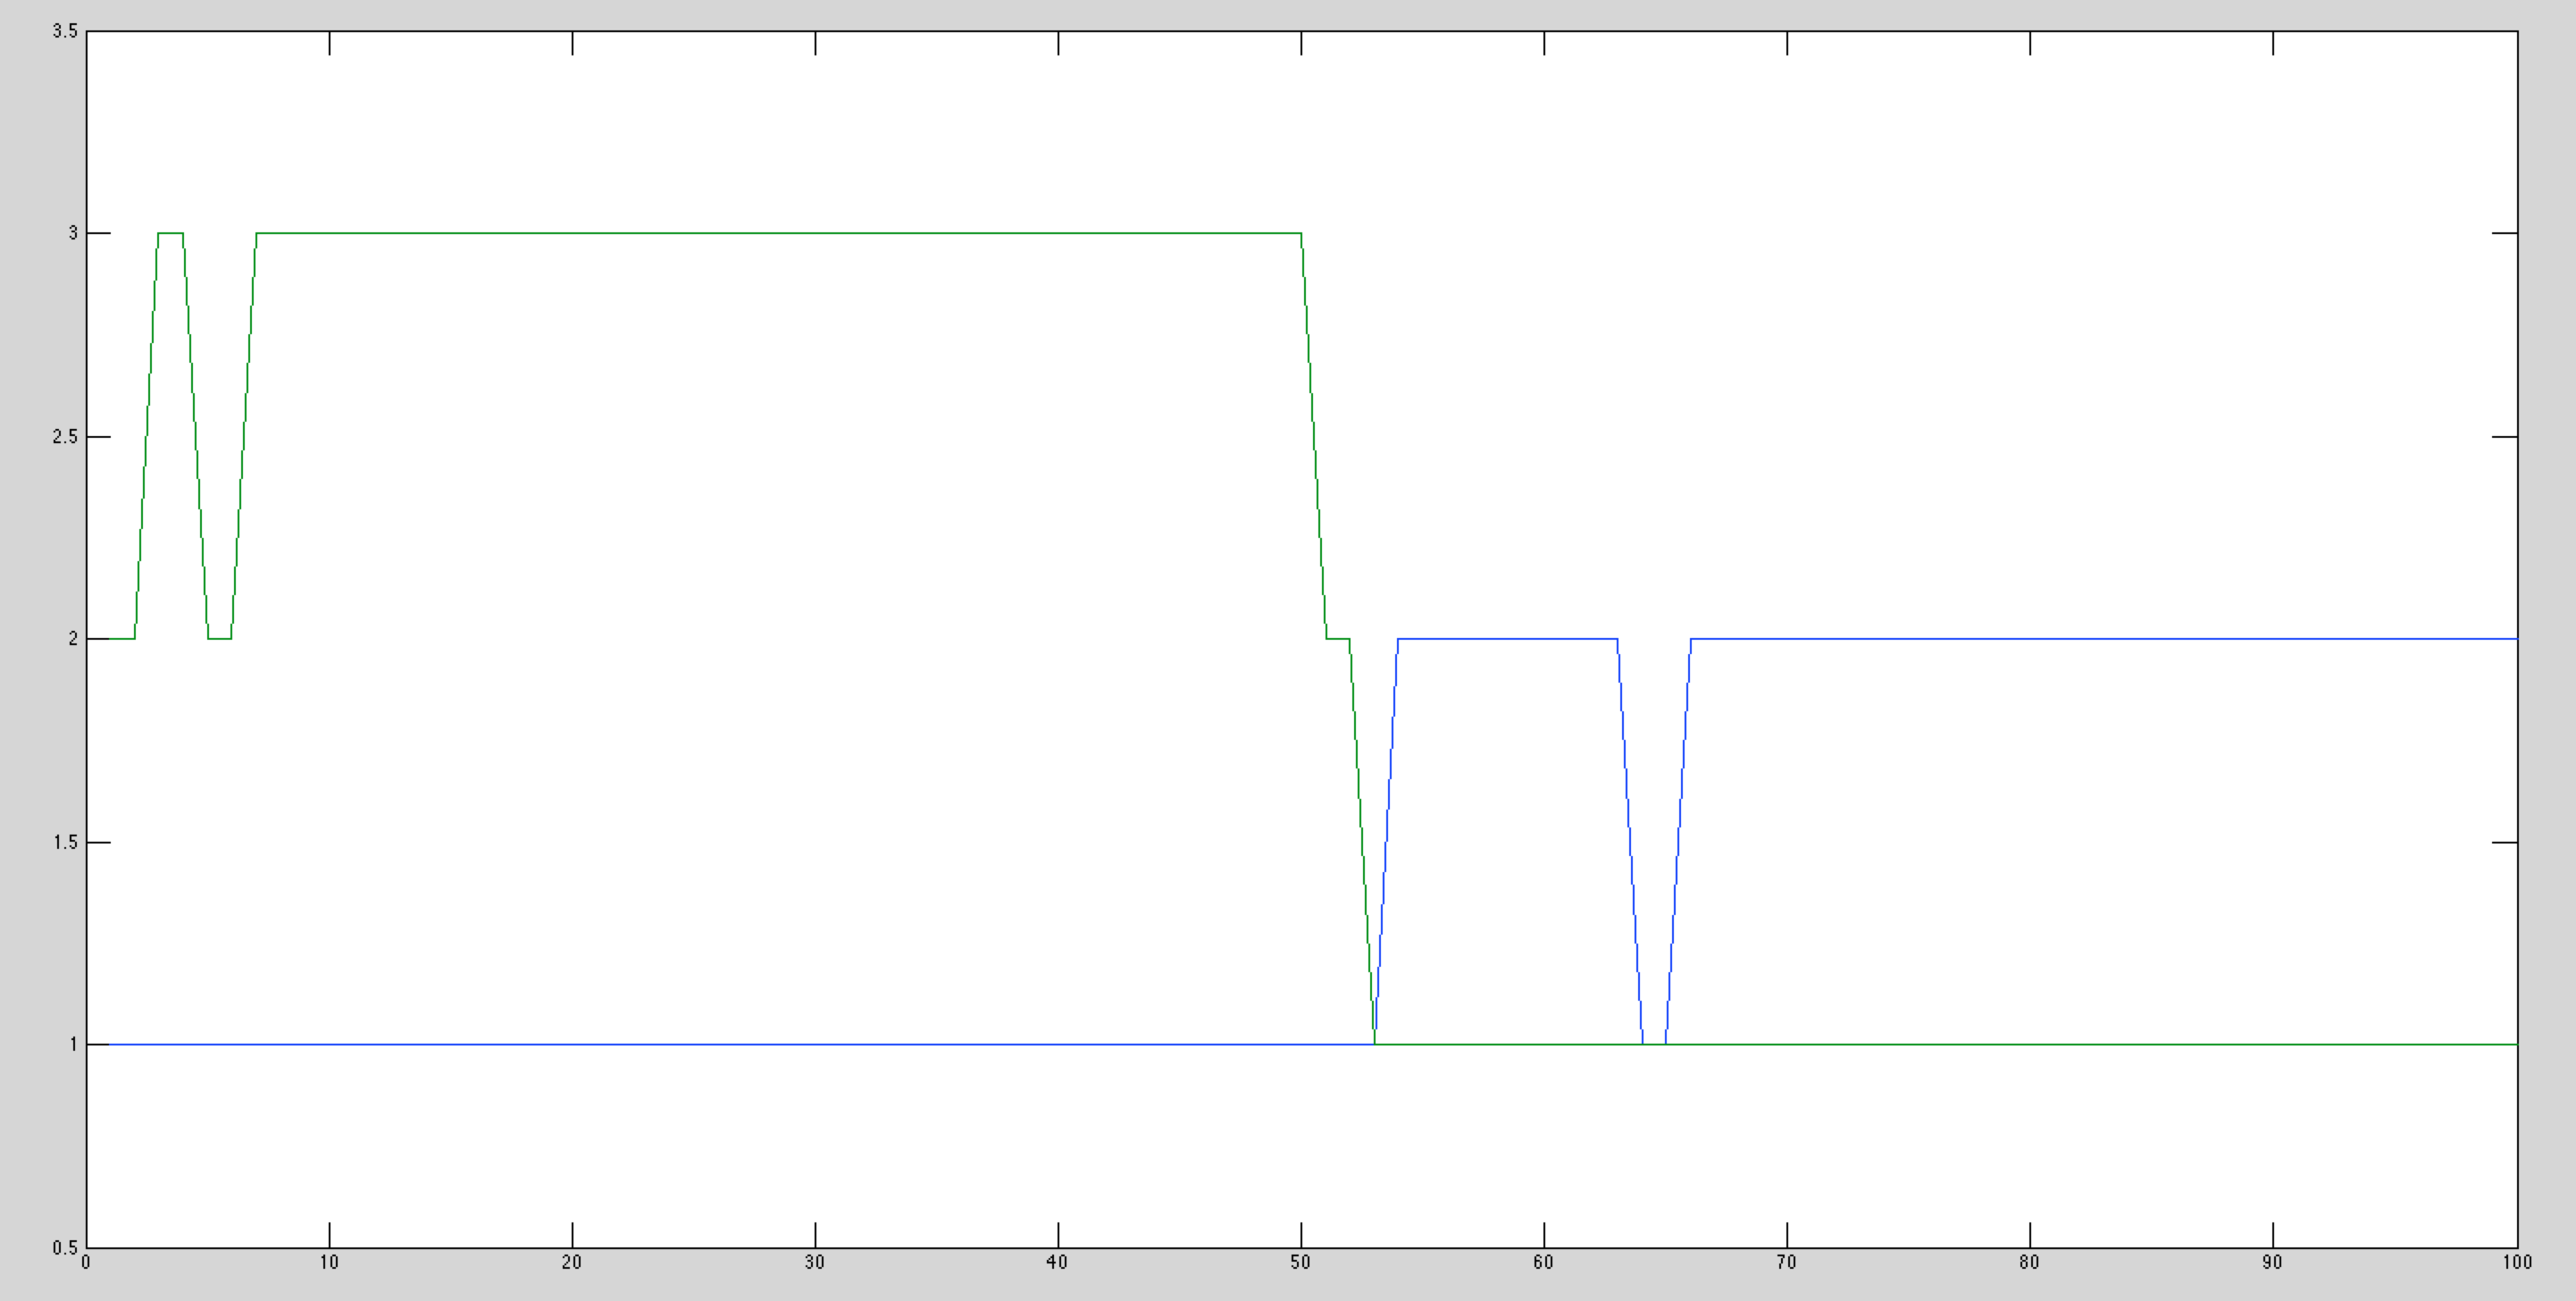
\includegraphics[width=14cm]{f2}
  \end{center}
  \end{figure}
  These are the two equilibria of the system.  Note that one can move from one to the other, but the probability of
  doing that is not just $\epsilon$, but $\epsilon^2$.  As $\tau\rightarrow0^+$ we can see the behavior approch one of
  these equilibrium and then stay there.  Which equilibrium depends entirely on where it starts.

  \item{Characterize the behavior of log-linear learning with Variation \#1 as $\tau\rightarrow 0^+$ for the
    above example.}\\
  In this strategy, players pick uniformly over their distrobutions which path they want to analyze, then calculate
  the log-linear strategy of that action versus the action they took last turn.  This strategy seems to play out
  exactly the same, quickly converging to one of the two NE.  In fact, if I run each algorithm thousands of times,
  both of them converge to $a_1b_3$ about 70\% of the time and $a_2b_1$ about 30\% of the time, where both games
  are given completely random starting points.  Additionally, almost every time variation \#2 would take much less
  changes before it settled down.  For instance, a typical run of variation \#1 going from $\tau=100$ to $\tau=1$ would
  look like:

  \begin{figure}[H]
  \begin{center}
  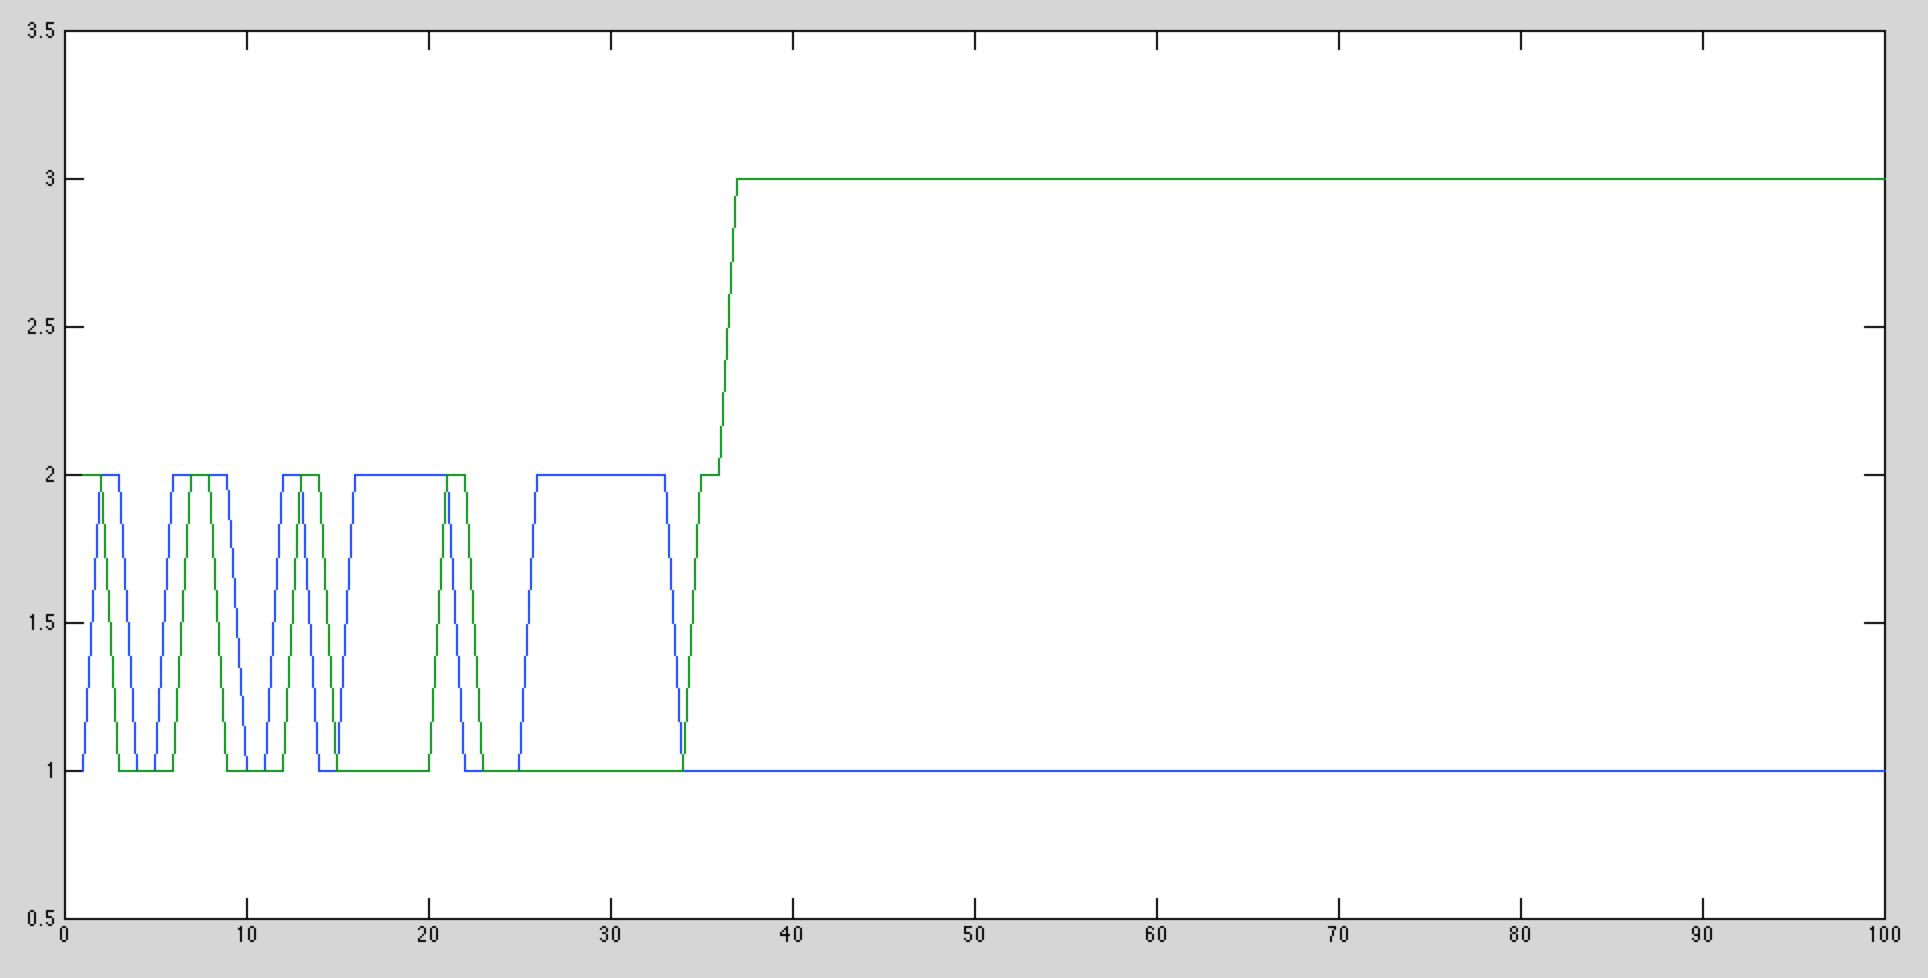
\includegraphics[width=14cm]{f3}
  \end{center}
  \end{figure}

  Whereas a typical run for variation \#2 would look like:

  \begin{figure}[H]
  \begin{center}
  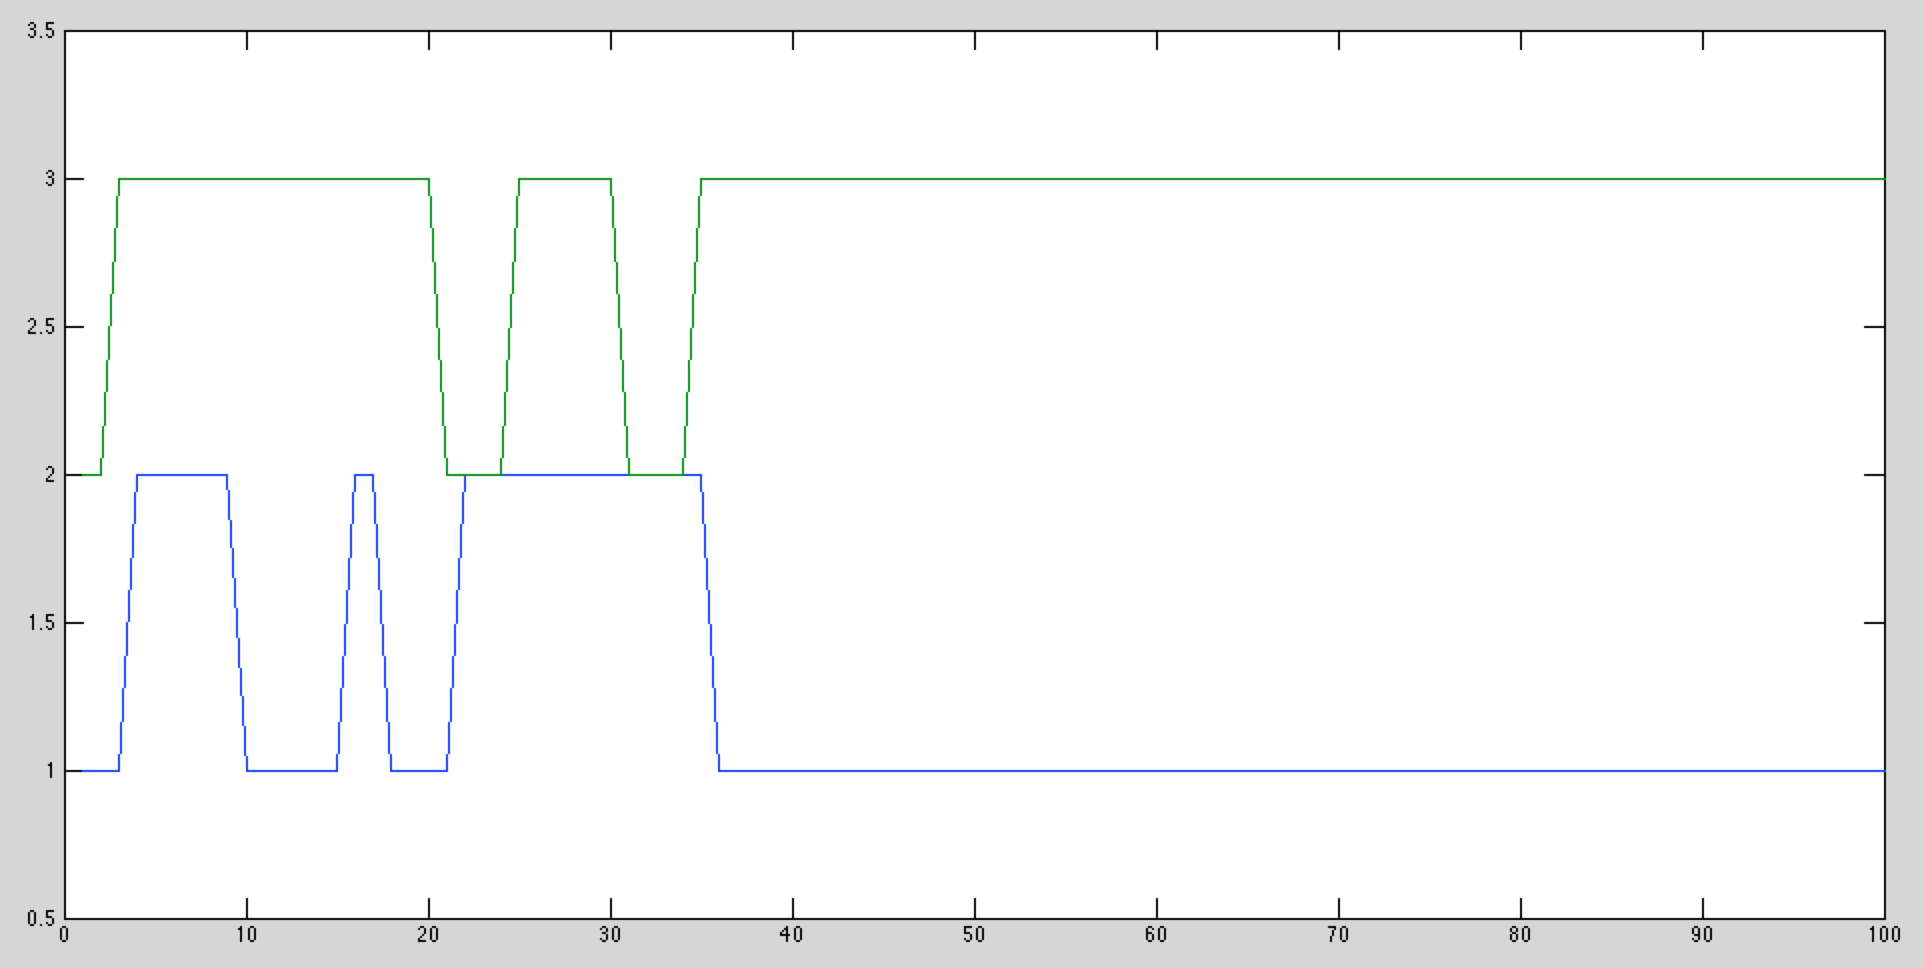
\includegraphics[width=14cm]{f4}
  \end{center}
  \end{figure}

  As you can see, there is a sort of inertia to variation \# 2.  This is because it takes into account the previous
  move.  If you are anywhere on the board, you have a uniform probability (1/3 or 1/2) to stay there.

  All of this code can be seen at the end of the test.

\end{enumerate}

\newpage
\textbf{2)} Consider the following class of resource allocation problems.
\begin{itemize}
  \item{A set of agents $N=\{1,2\}$}
  \item{A finite set of resources $\mathcal{R}=\{r_1,r_2,r_3\}$}
  \item{An anonymous welfare function for each resource $r$ of the form $W_r : \{0,1,2\}\rightarrow R$.
    The specific welfare functions are:}
  \[
    W_{r_1}(0)=0\text{, }W_{r_1}(1) = v_1\text{, }W_{r_1}(2)=1.5\cdot v_1
  \]
  \[
    W_{r_2}(0)=0\text{, }W_{r_2}(1) = v_2\text{, }W_{r_2}(2)=1.5\cdot v_2
  \]
  \[
    W_{r_3}(0)=0\text{, }W_{r_3}(1) = v_3\text{, }W_{r_3}(2)=1.5\cdot v_3
  \]
  where $v_1,v_2,v_3 \geq 0$ but unknown.
  \item{A finite action set of each player $\mathcal{A} \subseteq \mathcal{R}$.  Note that an action
    $a_i \in \mathcal{A}_i$ corresponds to just a single resource $r \in R$.  Let
    $\mathcal{A} := \mathcal{A}_1 \times \mathcal{A}_2$ represent the set of joint actions.}
  \item{A system-level welfare function of the form}
    \[
      W(a) = \sum_{r\in R}W_r(\abs{a}_r)
    \]
    Where $\abs{a}_r$ represents the number of players that chose resource $r$ in the action profile $a$, i.e.,
    \[
      \abs{a}_r = \abs{\{j\in N : r \in a_j\}}
    \]
\end{itemize}

The goal of this question is to understand how available utility design methodologies impact the
efficiency of the resulting pure Nash equlibria.

\begin{enumerate}[(a)]
  \item{Consider the special case where $\mathcal{A}_1=\mathcal{A}_2=\{r_1,r_2\}$ (i.e., no resource
    $r_3$ for this specific problem); However, $v_1$ and $v_2$ are unknown.  Suppose each agent is assigned
    marginal contribution utility.  What is the price of anarchy and price of stability of the class of games induced
    by the set of feasable values $v_1, v_2 \geq 0$.}\\

    We can imagine a case where both players are on seperate routes. In order for player 1 to leave his resource,
    $v_1<0.5\cdot v_2$.  For player 2 to leave, $v_2<0.5\cdot v_1$.  Now assume that we are on the same route.
    We imagine a situation on the edge, where $v_1=0.5 \cdot v_2$.  We would be at NE, but with a global welfare
    of:
    \[
      W(a) = 1.5 \cdot v_2 = 1.5\cdot 2\cdot v_1 = 3\cdot v_1
    \]
    In this same game, if they are both on different routes, the global welfare would be:
    \[
      W(a) = v_1+v_2 = v_1 + 2\cdot v_1 = 3\cdot v_1
    \]
    Meaning a PoA of:
    \[
      \frac{3\cdot v_1}{3\cdot v_1} = 1
    \]
    Well, the optimal path is the same as the NE, regardless of which of the two NE we are at in this game.
    We must now check on either side of thie inequality, first, if $v_1 < 0.5\cdot v_2$, then both players
    will play $v_2$ with a welfare function of:
    \[
      W(a) = 1.5\cdot v_2
    \]
    This is also the optimal, since the other payoff would be:
    \[
      W(a) = v_1 + v_2 < v_2 + 0.5\cdot v_2 \Rightarrow v_1+v_2 < 1.5\cdot v_2
    \]
    This is also a PoA of 1, since the optimal is the NE.  The only other case is when $v_1 > 0.5\cdot v_2$
    and $v_2 > 0.5\cdot v_1$.  The NE here is when the players are playing different resources, a welfare of:
    \[
      W(a) = v_1+v_2 > v_1 + \frac{1}{2}v_1 = 1.5\cdot v_1
    \]
    Again the NE is the optimal, a PoA of 1.  We have thus found:
    \[
      \text{PoA}=1\text{,  PoS}=1
    \]

  \item{Consider the special case where $\mathcal{A}_1=\{r_1,r_2\}$ and $\mathcal{A}_2=\{r_2,r_3\}$; however,
    $v_1$, $v_2$, and $v_3$ are unknown.  Suppose each agent is assigned the marginal contribution utility.  What
    is the price of anarchy and price of stability of the class of games induced by the set of feasable values
    $v_1,v_2,v_3\geq0$}

    This is much like the last game, except that we can have very poor NE.  For example, if $v_1=\frac{1}{2}v_2$
    and $v_3=v_2$.  In this case, player 1 could play $r_1$ and player 2 could play $r_2$.  No player would move
    because his new location would simply be the same payoff as before.  The optimal situation is if player 1 was
    on $r_2$ and player 2 was on $r_3$.  That would provide a welfare of $v_2+v_3 = 2\cdot v_2$.  The NE only
    provides a welfare of $v_1+v_2 = 1.5\cdot v_1$.  This means:
    \[
      \text{PoA}=\frac{4}{3}\text{,  PoS}=1
    \]
    PoS is 1 because in the last scenario, the optimum was another NE.  There is no worse situation, this is as bad as
    it gets.  This is because if $v_1$ was any higher, the PoA would still be positive, but it can only decrease.  if
    it was any lower, player 1 would move to $r_2$.  If $v_2$ was any higher, player 1 would move to it, if it was lower
    the PoA would drop.  If $v_3$ were any higher, player 2 would move to $r_3$.  If it were lower, PoA would drop.  In
    all of these situations, we either move to a new NE that is optimum, or the PoA drops.  Never do we increase PoA.

  \item{Consider the special case where $\mathcal{A}_1=\{r_1,r_2\}$ and $\mathcal{A}_2\{r_2,r_3\}$; however,
    $v_1$, $v_2$, and $v_3$ are unknown.  Suppose each agent is assigned the Shapley value utility.  What is the price of
    anarchy and price of stability of the class of games induced by the set of feasible values $v_1,v_2,v_3 \geq 0$.}

    We can imagine the same scenario as above.  Now the center point is only worth $0.75\cdot v_2$ for player 2, which means
    that he would rather play the full $v_2$ at $r_3$.  This means that the PoS for this game is 1, because for at least
    one game, the optimal is played.  Now imagine a different game, where $v_1=v_3$ and $v_1=\frac{4}{3}v_3$.  This is
    the edge point of this game, since at this point each player sees the same payoff at either action.  If they both play
    the same move then they will achieve a global welfare of $2v_3$.  If the both play middle, the will get the same
    global welfare.  If $r_1$ or $r_3$ was any larger, than that would be played by players 1 or 2 respectively.  In this
    case the global welfare would increase by the increase in that route, but that would now be the optimal welfare, since
    both players playing $r_2$ would remain the same   If $r_1$ or $r_3$ were to lower, than both players would play
    $r_2$ and would be achieving the optimal.  If $r_2$ were to increase, both players would play $r_2$.  If it were to
    decrease than both players would play their own respective chunks, which would be optimal.

    In simple terms, the shapley value utility is based only on the amount of players and their action sets, not on what
    is currently being played.  So there will always be only one equilibrium, and it will be optimal.  If there are more
    than one equilibrium they will all have the same global welfare.  We have:
    \[
      \text{PoA}=1\text{,  PoS}=1
    \]

\end{enumerate}

\newpage
\textbf{3)} Two players are to chose between two movies.  Player 1 (row) reads movie reads movie reviews
and has a better idea which one is better.  Player 2 (col) ignores movie reviews.  The player preferences
reflect a desire to see the better movie but also to go together.  This scenario may be described as a
Bayesian game as follows:
\begin{itemize}
  \item{States: $\omega_1$ and $\omega_2$}
  \item{State dependent payoff matricies:}
  \begin{center}
  \begin{tabular}{r |c|c|}
    \multicolumn{1}{r}{}
    & \multicolumn{1}{c}{A}
    & \multicolumn{1}{c}{B}\\
    \cline{2-3}
    A & 3,3 & 2,0 \\
    \cline{2-3}
    B & 0,2 & 1,1 \\
    \cline{2-3}
  \end{tabular}
  \begin{tabular}{r |c|c|}
    \multicolumn{1}{r}{}
    & \multicolumn{1}{c}{A}
    & \multicolumn{1}{c}{B}\\
    \cline{2-3}
    A & 1,1 & 0,2 \\
    \cline{2-3}
    B & 2,0 & 4,4 \\
    \cline{2-3}
  \end{tabular}\\
  \vspace{2mm}
  \hspace{8mm}$\omega_1$\hspace{2.5cm}$\omega_2$
  \end{center}
  \item{Types \& beliefs (i.e., Pr($\omega$) given type) over the states $\{\omega_1,\omega_2\}$:}
  \begin{itemize}
    \item{Player 1 (row) has 2 types, described by $t_1=\tau_1(\omega)$ as follows:}
      \begin{itemize}
        \item{$\tau_1(\omega_1) = \alpha$ with beliefs $\{2/3,1/3\}$}
        \item{$\tau_1(\omega_2) = \beta$ with beliefs $\{1/3,2/3\}$}
      \end{itemize}
    \item{Player 2 (col) has only 1 type, described by $t_2=\tau_2(\omega)$} as follows:
      \begin{itemize}
        \item{$\tau_2(\omega_1)=\tau_2(\omega_2) = (\alpha\beta)$ with beliefs $\{1/2,1/2\}$}
      \end{itemize}
  \end{itemize}
\end{itemize}
\begin{enumerate}[(a)]
  \item{Build the entire best response map for column player 2 (over pure strategies)}\\
    player 2 does not know that state, but believes that there is a $1/2$ probability that we
    are in any of these states.  We can find the payoffs for player 2 knowing this fact:
    \[
      U_2(AA) = \frac{1}{2}3 + \frac{1}{2}1 = 2
    \]
    \[
      U_2(AB) = \frac{1}{2}0 + \frac{1}{2}2 = 1
    \]
    \[
      U_2(BA) = \frac{1}{2}2 + \frac{1}{2}0 = 1
    \]
    \[
      U_2(BB) = \frac{1}{2}1 + \frac{1}{2}4 = 2\frac{1}{2}
    \]
    From this we can see the best responses for player 2:
    \[
      B_2(A) = \left( \begin{array}{c} 1 \\ 0 \end{array}\right), \text{ and } B_2(B) = \left( \begin{array}{c} 0 \\ 1 \end{array}\right)
    \]
    Player 2 will always choose to see the same movie as player 1.

  \item{Derive all Bayes-Nash equilibria (over pure strategies)}
    Player 1 know some information about what state he is in, but he still does not have all the information.
    We can find his payoffs when given signal $\alpha$:
    \[
      U_{1\alpha}(AA) = \frac{2}{3}3 + \frac{1}{3}1 = 2\frac{1}{3}
    \]
    \[
      U_{1\alpha}(AB) = \frac{2}{3}2 + \frac{1}{3}0 = 1\frac{1}{3}
    \]
    \[
      U_{1\alpha}(BA) = \frac{2}{3}0 + \frac{1}{3}2 = \frac{2}{3}
    \]
    \[
      U_{1\alpha}(BB) = \frac{2}{3}1 + \frac{1}{3}4 = 2
    \]
    when given signal $\beta$:
    \[
      U_{1\beta}(AA) = \frac{1}{3}3 + \frac{2}{3}1 = 1\frac{2}{3}
    \]
    \[
      U_{1\beta}(AB) = \frac{1}{3}2 + \frac{2}{3}0 = \frac{2}{3}
    \]
    \[
      U_{1\beta}(BA) = \frac{1}{3}0 + \frac{2}{3}2 = 1\frac{1}{3}
    \]
    \[
      U_{1\beta}(BB) = \frac{1}{3}1 + \frac{2}{3}4 = 3
    \]

    Alright, now we can move through action profiles to check if they are equilibria:
    \begin{itemize}
      \item{\{(A,A),A\}: Player 2 is obviously happy, recieving a payoff of 2, player 1 also recieves
        a payoff of $(2\frac{1}{3},1\frac{2}{3})$ which is better than the alternatives of $\frac{2}{3}$
        and $1\frac{1}{3}$ respectively.}
      \item{\{(A,A),B\}: Player 2 would rather play A.}
      \item{\{(A,B),A\}: Player 1 would rather play (A,A)}
      \item{\{(A,B),B\}: Player 1 would rather play (B,B)}
      \item{\{(B,A),A\}: Player 1 would rather play (A,A)}
      \item{\{(B,A),B\}: Player 1 would rather play (B,B)}
      \item{\{(B,B),A\}: Player 2 would rather play B.}
      \item{\{(B,B),B\}: Player 2 is happy, getting his highest possible payoff.  Player 1 is getting
        $(2,3)$, Which is better than $1\frac{1}{3}$ and $\frac{2}{3}$.}
    \end{itemize}

    We have shown that the only two NE are \{(A,A),A\} and \{(B,B),B\}

\end{enumerate}


\newpage
Variation \#1
\begin{figure}[H]
\begin{center}
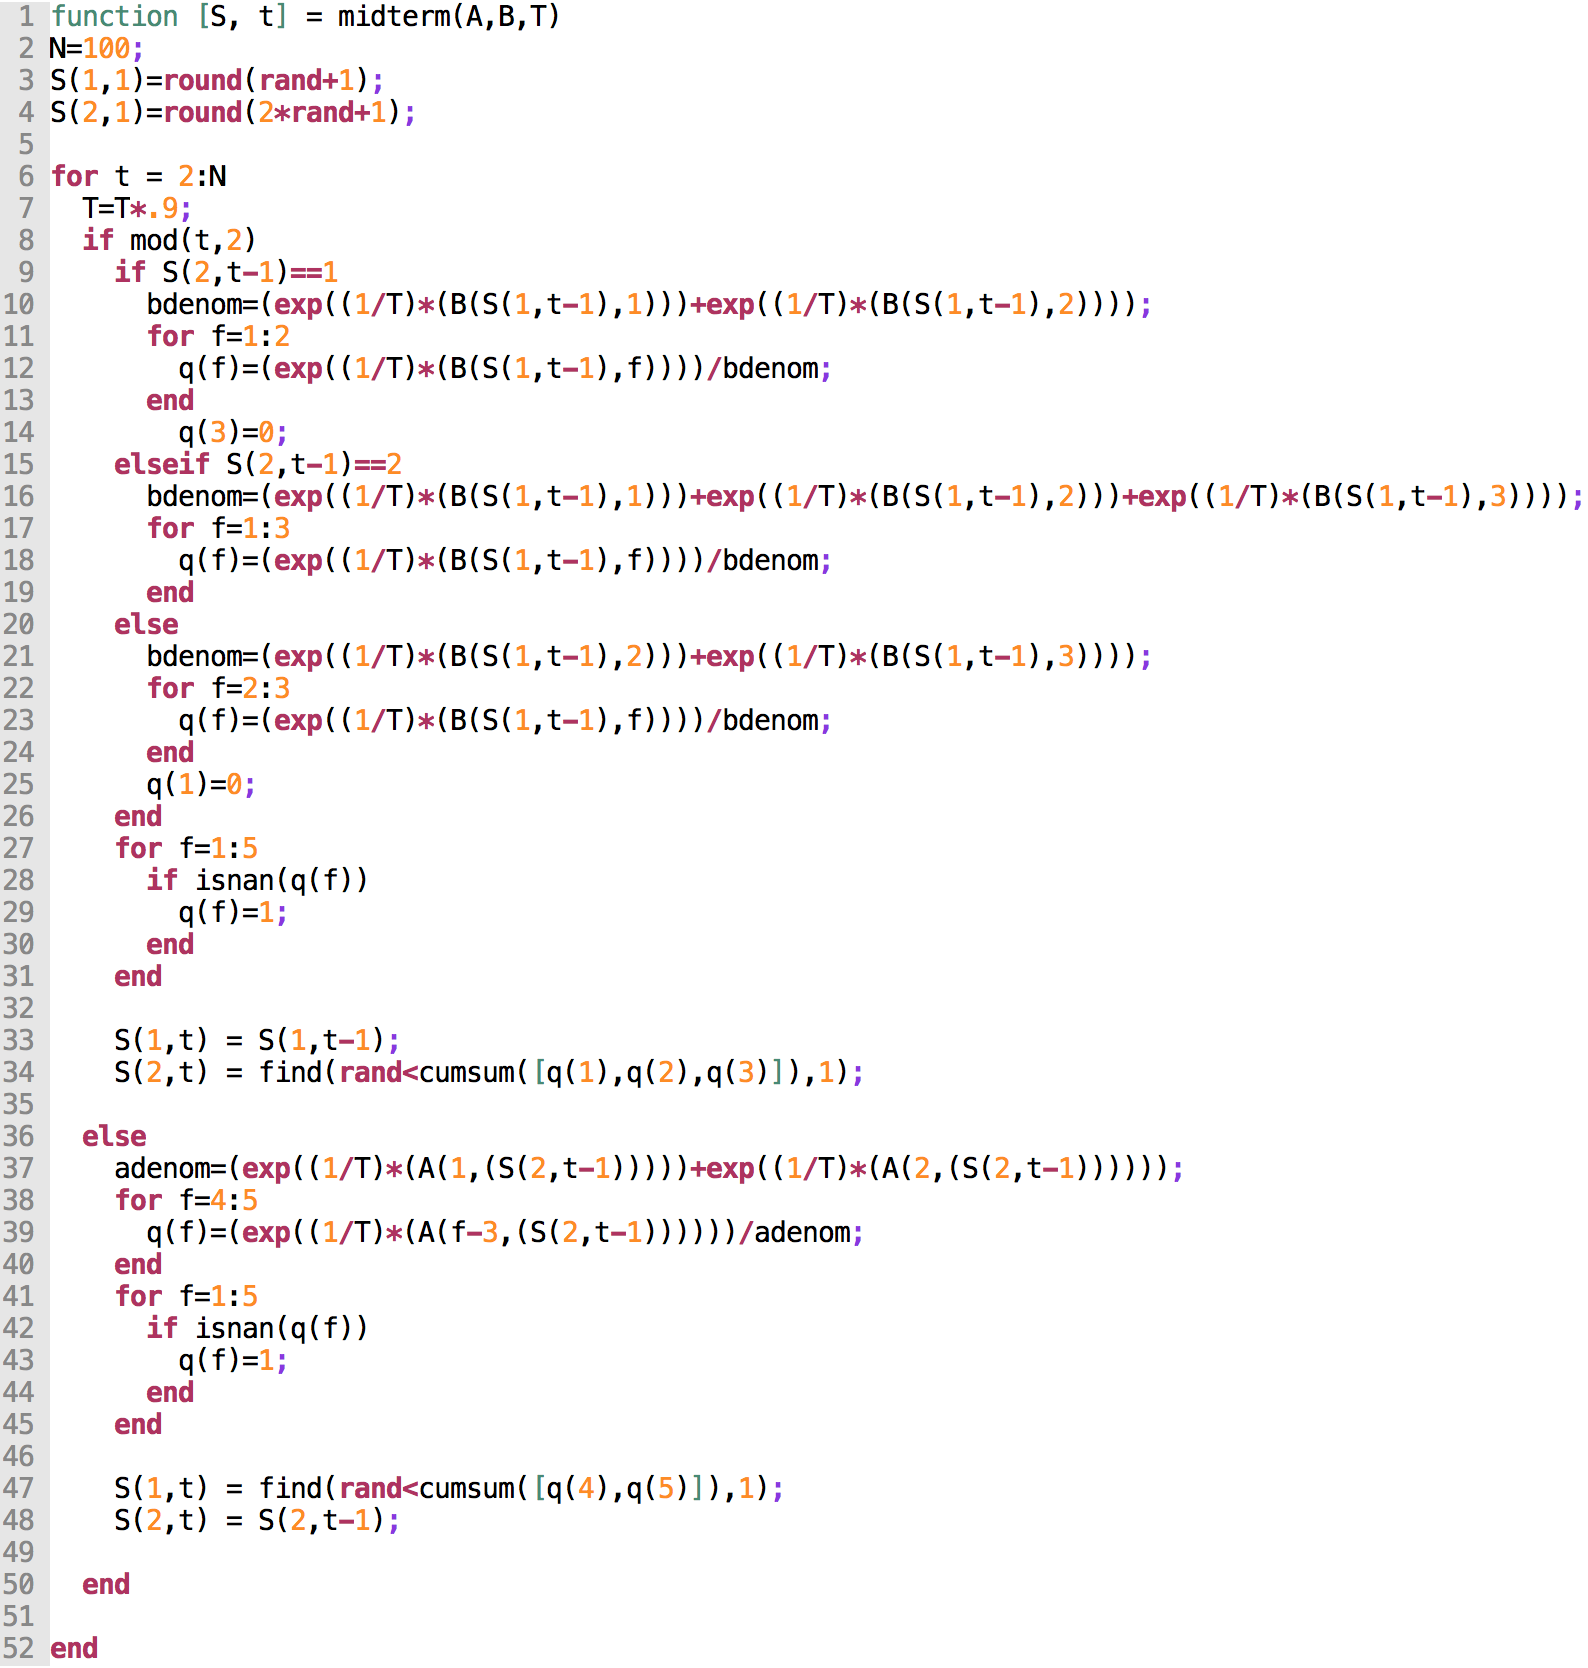
\includegraphics[width=14cm]{f5}
\end{center}
\end{figure}
\newpage
Variation \#2
\begin{figure}[H]
\begin{center}
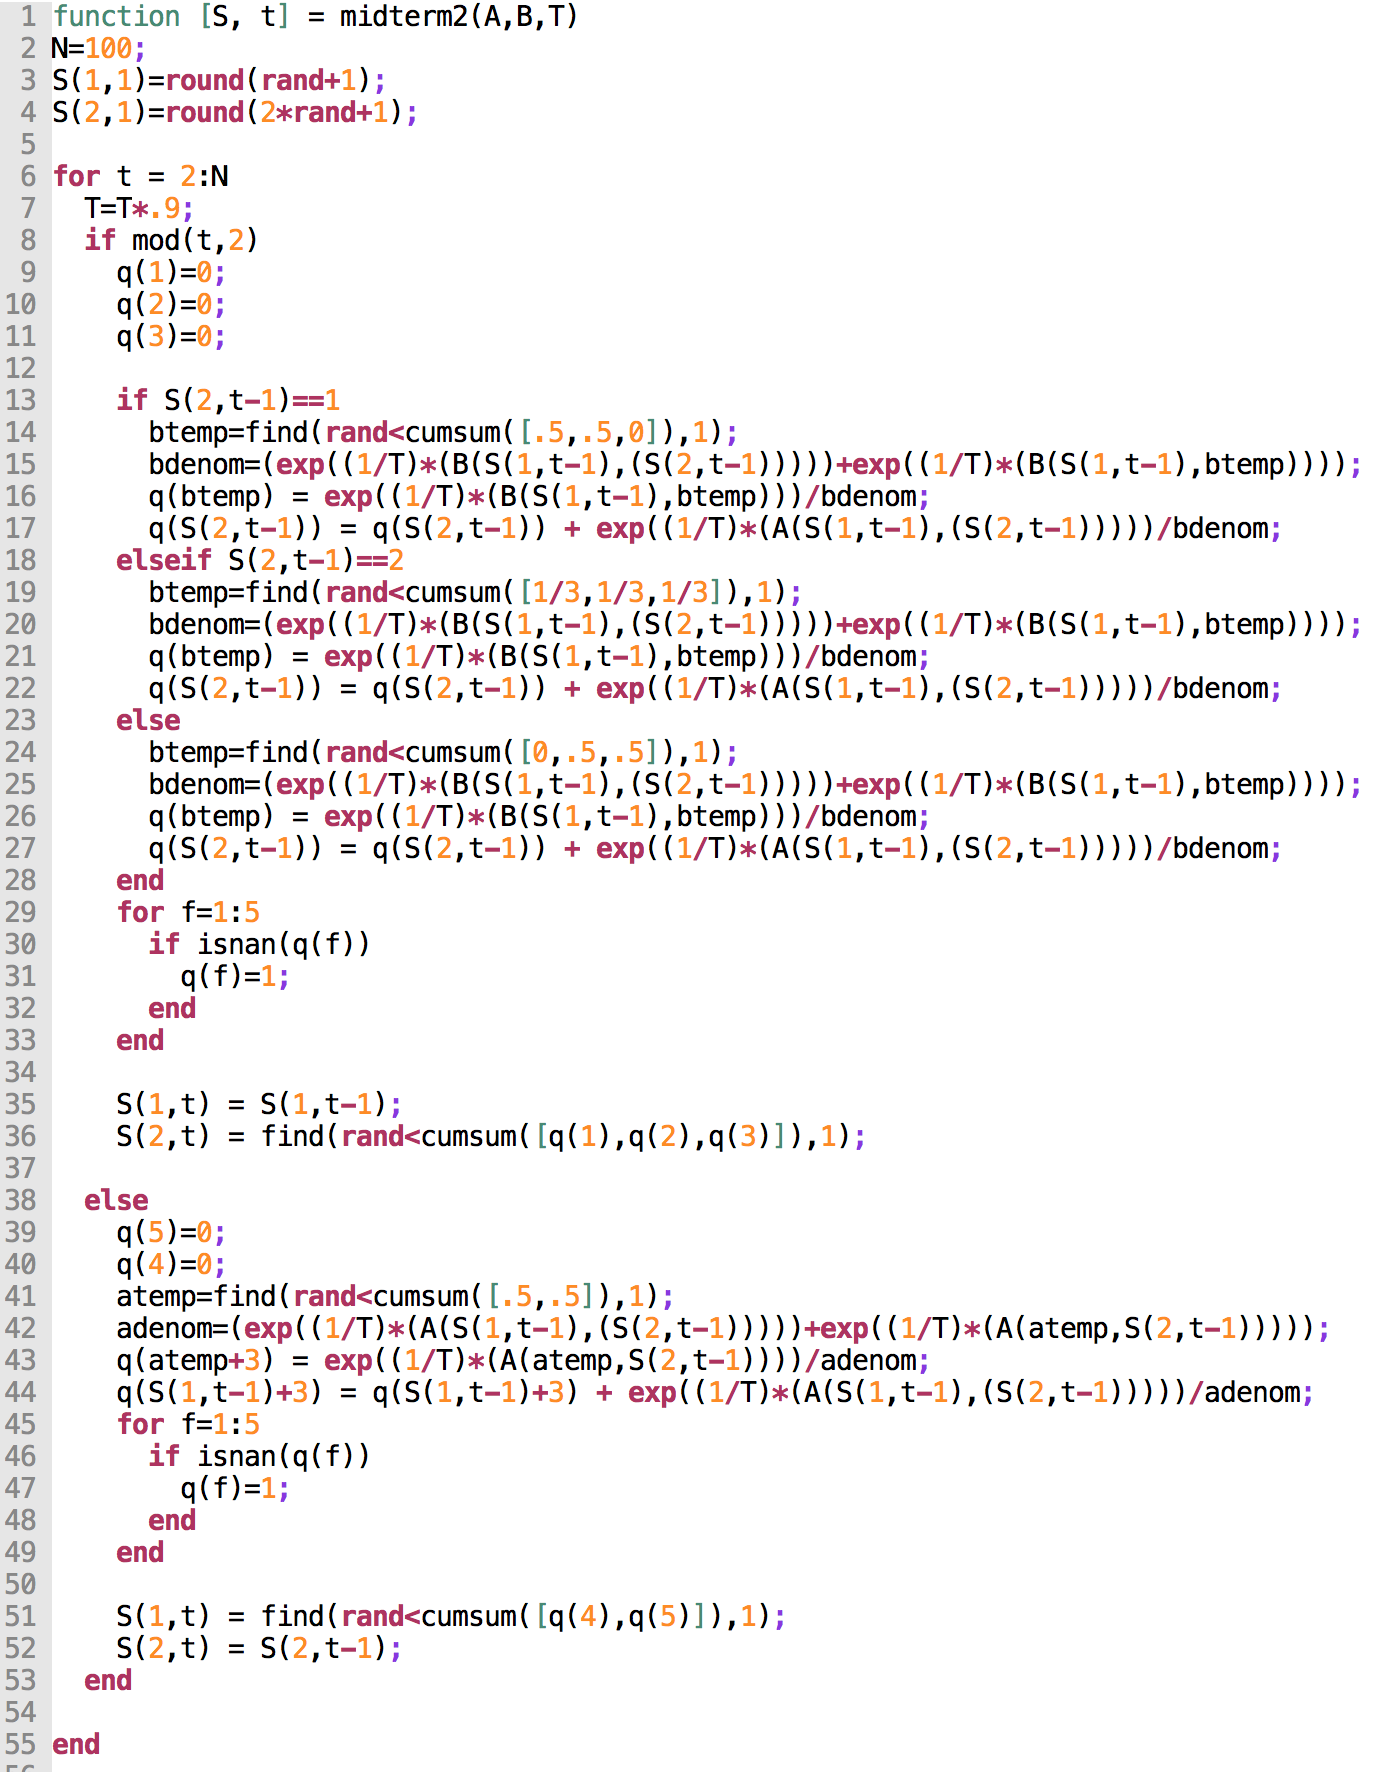
\includegraphics[width=13cm]{f6}
\end{center}
\end{figure}


\end{document}
